\documentclass[11pt,a4paper,english]{article}
\usepackage[english]{babel} % Using babel for norwegian hyphenation
\usepackage{lmodern} % Changing the font
\usepackage[utf8]{inputenc}
\usepackage[T1]{fontenc}

%\usepackage[moderate]{savetrees} % [subtle/moderate/extreme] really compact writing
\usepackage{tcolorbox}
\usepackage[parfill]{parskip} % Removes indents
\usepackage{amsmath} % Environment, symbols etc...
\usepackage{amssymb}
\usepackage{float} % Fixing figure locations
\usepackage{multirow} % For nice tables
%\usepackage{wasysym} % Astrological symbols
\usepackage{graphicx} % For pictures etc...
\usepackage{enumitem} % Points/lists
%\usepackage{physics} % Typesetting of mathematical physics examples: \bra{}, \ket{}, expval{}
\usepackage{url}

\definecolor{red}{RGB}{255,10,10}

% To include code(-snippets) with æøå
\usepackage{listings}
\lstset{
language=c++,
showspaces=false,
showstringspaces=false,
frame=l,
}

\tolerance = 5000 % Bedre tekst
\hbadness = \tolerance
\pretolerance = 2000

\numberwithin{equation}{section}

\newcommand{\conj}[1]{#1^*}
\newcommand{\ve}[1]{\mathbf{#1}} % Vektorer i bold
\let\oldhat\hat
\renewcommand{\hat}[1]{\mathbf{\oldhat{#1}}}
\newcommand{\trans}[1]{#1^\top}
\newcommand{\herm}[1]{#1^\dagger}
%\renewcommand{\thefootnote}{\fnsymbol{footnote}} % Gir fotnote-symboler
\newcommand{\Real}{\mathbb{R}}
\newcommand{\bigO}[1]{\mathcal{O}\left( #1 \right)}

\newcommand{\spac}{\hspace{5mm}}

\title{FYS3150/4150\\Computational Physics\\Project 1}
\author{Magnus Ulimoen\\Krister Stræte Karlsen}
\date{\today}

\begin{document}
\maketitle

\section{Introduction}

A great deal of differential equations in the natural sciences can be written 
as a linear second-order differential equation on the form
\begin{equation}
\frac{d^y}{dx^2} + k^2(x)y = f(x)
\label{eq:2orderDIFF}
\end{equation}

Some examples include, Schrödinger's equation, the Airy function,
Poisson's equation and a special case, Laplace's equation.

Being able to solve such equations optimally with respect to accuracy 
and efficiency is undoubtedly important. This report will compare 
different algorithms for solving them.

The algorithms to be investegated in this report are	 standard Gaussian 
Elimination, LU decomposition, sparse matrix decomposition and an 
algorithm specifically tailored for a tridiagonal system of 
linear equations. 


\subsection{A closer look at an example from Electromagnetism}

In electrostatics Maxwells equations reduces to
\begin{gather}
\nabla \cdot \ve{E} = \frac{\rho}{\epsilon_0}\\
\nabla \cdot \ve{B} = 0\\
\nabla \times \ve{E} = 0\\
\nabla \times \ve{B} = 0
\end{gather}
As the curl of the electric field is zero, the field is conservative
and can be written on the form
\begin{equation}
\nabla \Phi = -\ve{E}
\end{equation}
This gives Poisson's equation
\begin{equation}
\nabla^2\Phi = -\frac{\rho(\ve{r})}{\epsilon_0}
\end{equation}

Letting $\rho$ be spherically symmetric leads to a symmetric $\Phi$.
This gives with a substitution $\Phi(r) = \phi(r)/r$
\begin{equation}
\frac{d^2\phi}{dr^2} = -\frac{r\rho(r)}{\epsilon_0}
\end{equation}
Which is on the form of \eqref{eq:2orderDIFF} with $k(x)=0$, which is also the differential
equation which is solved in this paper.

\section{Method}

The specific differential equation, with boundery values, being discussed in this report is: 

\begin{equation}
-u''(x) = f(x), \spac x \in [0,1], \spac u(0) = u(1) = 0.
\end{equation}

This boundery value problem can be discretized and written as a system of linear equations.

Letting the domain $x \in [0,1]$ be discretized into $n+2$ pieces,
\begin{gather}
x_0, x_1, \dots, x_{n}, \dots, x_{n+1}
\end{gather}
where 
\begin{gather}
h = \frac{x_{n+1} - x_0}{n+1} = \frac{x_{n+1}}{n+1}\\
x_i = x_0 + ih = ih
\end{gather}

an then sampling the solution at the mesh points so that $u(x_i) \simeq v_i$.

And using the three-point formula from the symmetric 
Taylor-expansion for the second derivative of v,
\begin{equation}
\frac{d^2v}{dx^2} \simeq \frac{v_{i-1} + v_{i+1} - 2v_i}{h^2}
\end{equation}

The discretized form of equation (2.1) can then be written as
\begin{gather}
\frac{v_{i-1} + v_{i+1} - 2v_i}{h^2} = \tilde{f}_i , \quad i=1,2, \dots, n 
\end{gather}
with $\tilde{f}_i = f(r_i) h^2$.

With boundary conditions 
\begin{gather}
v_0 = v_{n+1} = 0
\end{gather}

This can now be written as a system of linear equations on the form 

\begin{equation}
   \ve{A}\ve{v} = \tilde{\ve{b}},
   \label{eq:Avb}
\end{equation}

Multipling the discretized equation (2.6) by $h^2$ we get:

\begin{gather*}
   -v_{i-1}+2v_{i}-v_{i+1}=h^2 f_i \hspace{0.5cm} \mathrm{for} \hspace{0.5cm} i=1,\dots, n 
\end{gather*}

Filling in for $i$ and choosing $\tilde{b_i} = h^2 f_i$ we obtain the following set of equations: 
\begin{align*}
	2v_{1}-v_{2}=\tilde{b_1} \\
	-v_{1}+2v_{2}-v_{3}=\tilde{b_2} \\
	\vdots \hspace{0.5cm} \\
	-v_{i-1}+2v_{i}-v_{i+1}=\tilde{b_i} \\
	\vdots \hspace{0.5cm}  \\ 
	-v_{n-1}+2v_{n}=\tilde{b_n} \\
\end{align*}
Now one can easily see that this system of linear equations can written on the form of \eqref{eq:Avb}
\begin{gather*}
    \ve{A} = \begin{pmatrix}
                           2& -1& 0 &\dots   & \dots &0 \\
                           -1 & 2 & -1 &0 &\dots &\dots \\
                           0&-1 &2 & -1 & 0 & \dots \\
                           & \dots   & \dots &\dots   &\dots & \dots \\
                           0&\dots   &  &-1 &2& -1 \\
                           0&\dots    &  & 0  &-1 & 2 \\
                      \end{pmatrix},\spac \ve{v} = \begin{pmatrix}
                           v_0\\
                           v_1\\
                           \dots \\
                          \dots  \\
                          \dots \\
                           v_{n-1}\\
                      \end{pmatrix},
  \spac \tilde{\ve{b}} = \begin{pmatrix}
                           \tilde{b}_0\\
                           \tilde{b}_1\\
                           \dots \\
                           \dots \\
                          \dots \\
                           \tilde{b}_{n-1}\\
                      \end{pmatrix}.
\end{gather*}

Having a complete set of linear equations we move on to how to solve them.

\subsection{A tridiagonal matrix algorithm}
\label{subsec:Thomas}

We start by looking at the system of equations:
\begin{align}
	 b_1 v_1 + c_1 v_{2} = \tilde{b_1} \label{eq:1star}\\
	 a_2 v_1 + b_2 v_2 + c_3 v_3 = \tilde{b_2} \label{eq:2star}\\
	 a_3 v_2 + b_3 v_3 + c_3 v_4 = \tilde{b_3} \label{eq:3star}\\
\nonumber\vdots \hspace{0.5cm}  \\ 
	 a_n v_{n-1} + b_n v_n = \tilde{b_n} \label{eq:Nstar}
\end{align}
If we solve \eqref{eq:1star} for $v_1$ and insert it into \eqref{eq:2star} we obtain the following "modified second equation":
\begin{align*}
	(b_1 b_2 - a_2 c_1)v_2 + b_1 c_2 v_3 = b_1 \tilde{b_2} - a_2  \tilde{b_1}  
\end{align*}
Now having successfully removed $v_1$ from the second equation we can go on and solve it for $v_2$ and insert it into the third equation obtaining:
\begin{align*}
(b_3 (b_1 b_2 - a_2 c_1)- a_3 b_1 c_2)v_3 + c_3(b_1 b_2 -a_2 c_1)v_4 = \\
(b_1 b_2 - a_2 c_1 ) \tilde{b_3} - a_3 b_1 \tilde{b_2} + a_2 a_3 \tilde{b_1} 
\end{align*}

The two modified equations may be written as 

\begin{align*}
v_2 = \frac{b_1 \tilde{b_2} - a_2 \tilde{b_1}}{b_1 b_2 - a_2 c_1} - \frac{b_1 c_2}{b_1 b_2 - a_2 c_1} v_3 = \beta_2 + \gamma_2 v_3
\end{align*}
\begin{align*}
v_3 =& \frac{(b_1 b_2 - a_2 c_1) \tilde{b_3} - a_3 (b_1 \tilde{b_2} - a_2 \tilde{b_1})}{b_3 (b_1 b_2 - a_2 c_1)- a_3 b_1 c_2} - \frac{c_3(b_1 b_2 - a_2 c_1)}{b_3 (b_1 b_2 - a_2 c_1)- a_3 b_1 c_2} v_4 \\
=&  \frac{\tilde{b_3}-a_3 \beta_2}{a_3 \gamma_2 + b_3} + \frac{-c_3}{a_3 \gamma_2 + b_3}v_4 = \beta_3 + \gamma_3 v_4
\end{align*}

This prossess can be repeated up untill the last equation. 
This is the forward substitution step. 
From the last equation we compute $v_n$ and get all we need to compute $v_{n-1}$,
then $v_{n-2}$, and so on. This is the backward substitution part of the algorithm. A shrewd reader might see that the coefficiants, $\beta$ and $\gamma$, take a recursive form
\begin{align*}
\beta_{i} = \frac{\tilde{b_i}-a_i \beta_{i-1}}{a_i \gamma_{i-1} + b_i} , \hspace{0.5cm} \gamma_{i}=\frac{-c_i}{a_i \gamma_{i-1} + b_i},
\end{align*}
and the equation for $v_{i-1}$ reads: 
\begin{equation}
v_{i-1} = \beta_{i-1} + \gamma_{i-1} v_i
\label{eq:viminus1}
\end{equation}

It follows from \eqref{eq:1star} that $\beta_1 = \frac{\tilde{b_1}}{b_1}$ and $\gamma_1 = \frac{-c_1}{b_1}$.
From combining \eqref{eq:Nstar} and \eqref{eq:viminus1} we get 
\begin{align*}
v_n = \frac{\tilde{b_n}-a_n \beta_{n-1}}{a_n \gamma_{n-1} + b_n} = \beta_{n}.
\end{align*}

Having all the nessecary ingredients the algorithm reads as follows.
\vspace{0.5cm}

\centerline{Algorithm I}
\begin{tcolorbox}
$a_i = c_i = -1, \hspace{0.5cm}  i=1,2,3,..,n$\\
$b_i = 2, \hspace{0.5cm}  i=1,2,3,..,n $\\
$\tilde{b_i} = h^2 f_i \hspace{0.5cm}  i=1,2,3,..,n $\\
$\beta_1 = \frac{\tilde{b_1}}{b_1}$ \\
$\gamma_1 = \frac{-c_1}{b_1}$ \\
for $i=2,3,..,n$ \\ \vspace{0.5cm} 
 \hspace{0.5cm} $ \beta_{i} = \frac{\tilde{b_{i-1}}-a_{i-1} \beta_{i-1}}{a_{i-1} \gamma_{i-1} + b_{i-1}} , \hspace{0.5cm} \gamma_{i}=\frac{-c_{i-1}}{a_{i-1} \gamma_{i-1} + b_{i-1}} $ \vspace{0.2cm}  \\
 $v_{n} = \beta_{n}$\\
for $i=n, n-1, \cdots ,2$\\ \vspace{0.5cm} 
 \hspace{0.5cm} $v_{i-1} = \beta_{i-1} + \gamma_{i-1} v_i$
\end{tcolorbox} 


This is often refered to as \emph{Thomas Algorithm}, or \emph{TDMA}, an algorithm for solving tridiagonal systems of linear equations. 

\subsubsection{FLOPS}
This algorithm requires nine operations for each row for the forward substitution,
and two backwards. This requires 11 FLOPS for each row to solve the system.
With n rows this algorithm requires 11N FLOPS.

In big O notation the complexity of $\bigO{n}$.

\subsubsection{Implementation}

The algorithm in section \ref{subsec:Thomas} is implemented in C++.
Since we do not have changing $a_i$ we have coded $a_i = a$.
The zero-indexing in C++ is used, and the elements accessed in the code
is different from the algorithm.

\subsection{Standard Gaussian Elimination}

The Gaussian elimination is solving the system \eqref{eq:Avb} by using 
row operations and getting a row echelon form and then backsubstituting.

This operation in principle is here shown for matrix A.
\begin{gather}
A = \begin{pmatrix}
    a_{11} & a_{12} & a_{13} & \cdots & y_1\\
    a_{21} & a_{22} & a_{23} & \cdots& y_2\\
    a_{31} & a_{32} & a_{33} & \cdots & y_3\\
    \cdots \\
    a_{n1} & a_{n2} & \cdots & & y_n
    \end{pmatrix}
\end{gather}

To get the matrix into the row echelon the first row needs to have a non-zero
value as its first element. Then a constant $c_i = a_{i1}/a_{11}$ is 
calculated, and a subtraction of the first row,
\begin{gather}
a_{ij} = a_{ij} - c_i a_{ij}
\end{gather}
is done. For the elements $a_{i1}$, this gives zero, and the matrix is
row reduced to
\begin{gather}
A \sim
\begin{pmatrix}
    a_{11} & a_{12} & a_{13} & \cdots\\
    0 & a_{22} - c_2 a_{22} & a_{23} - c_2 {a}_{23} & \cdots\\
    0 & a_{32} - c_3 a_{32} & a_{33} - c_3 a_{33} & \cdots\\
    0 & \cdots \\
    0 & a_{n2} - c_2 a_{n2} & \cdots
\end{pmatrix}
\end{gather}
The operation can be repeated on the submatrix $A_{(2-N)(2-N)}$
until the decired triangular matrix is achieved.

The backsubstitution is simple when a row reduced matrix is achieved,
by examining the matrix equation $\ve{U}\ve{x} = \ve{\tilde{y}}$
\begin{gather}
\begin{pmatrix} u_{11} & u_{12} & \dots\\
                0 & u_{22} & u_{23} & \dots\\
                &\dots & \dots\\
                0 & \dots & a_{(n-1)(n-1)} & a_{(n-1)n} \\
                & \dots & 0 & a_{nn}
\end{pmatrix} \begin{pmatrix} x_1 \\ x_2 \\ \dots \\ x_{n-1}\\ x_n \end{pmatrix}
 = \begin{pmatrix} \tilde{y}_1 \\ \tilde{y}_2 \\ \dots\\ \tilde{y}_{n-1} \\ \tilde{y}_n \end{pmatrix}\\
 x_n = \frac{\tilde{y}_n}{a_{nn}}\\
 x_{n-1} = \frac{\tilde{y}_{n-1} - a_{(n-1)n}x_n}{a_{(n-1)(n-1)}}
\end{gather}
Where $x_{i}$ is found from a recursive method extended from this.

\subsubsection{FLOPS}
For a general matrix with size ($N\times N$), the algorithm requires
$N^2$ operations per row reduction. This is repeated for all N rows,
and the complexity is $\bigO{n^3}$ for the reduction. The backwards 
substitution has $\bigO{n^2}$ and is not of significance.



\subsubsection{Implementation}
\label{subsubsec:impl_gauss}
The matrix solvers are used from the Armadillo 
library\footnote{\url{http://arma.sourceforge.net/}}. The matrix is
created by indexing the non-zero elements and setting this equal to the 
tridiagonal elements. The calculation is done by a call to 
\begin{lstlisting}
arma::Col<double> x = solve(A, b);
\end{lstlisting}
Which returns the resulting vector.

\subsection{LU decomposition}

The matrix $\ve{A}$ can be decomposited into an upper triangular matrix $\ve{U}$ and 
a lower triangular matrix $\ve{L}$. The elements on the diagonal of $\ve{L}$ are 1,
and it is invertible.

By decomposition the result is
\begin{gather}
\ve{Ax} = \ve{LUx} = \ve{w}
\end{gather}
Which is then solved for $\ve{x}$ by using a the inverse of $\ve{L}$
\begin{gather}
\ve{Ux} = \ve{L^{-1}w} = \ve{y}.
\end{gather}
Since $\ve{U}$ is an upper triangular matrix the solution is found from back-substitution
of the elements as described in the Gaussian Elimination.

\subsubsection{FLOPS}
The decomposition into the LU-matrix requires $\bigO{N^3}$ FLOPS, but 
has the advantage that backwards substitution just requires $\bigO{N^2}$
FLOPS to compute. This decomposition is also highly reusable if \eqref{eq:Avb}
is to be solved for more than one $\ve{x}$, or the determinant is to be found.

\subsubsection{Implementation}

The LU decomposition is achieved with the Armadillo library, by calling
the lu()-method. This produces three matrices, $\ve{L}$, $\ve{U}$ and a transformation
matrix $\ve{P}$, such that
\begin{gather}
\ve{A} = \ve{ \trans{P}LU }
\end{gather}
The vector y is then created by
\begin{gather}
\ve{y} = \left( \ve{ \trans{P}L }  \right)^{-1}
\end{gather}
Then the solver function in the Armadillo library is used.

\subsection{Method using sparse}

To prevent saving a very sparse matrix in memory a sparse method can be employed.
This saves the non-zero matrix elements and location instead of the 
entire matrix. This saves memory and computational speed, as only these
elements are manipulated.

\subsubsection{FLOPS}

For a sparse matrix (with suitable algorithms) the number of operations are considerably
less than for the Gaussian reduction when the matrices are sparse.
The amount of computations is very dependent upon the nature of the matrix.

\subsubsection{Implementation}

For our very sparse matrix which has $N-3$ unused elements per row, the
memory-space saved is $(N-3)^2$. This helps keep the matrix in the 
CPU-cache and speeds it up for larger matrices. The implementation follows
from the non-sparse solver, but a sparse matrix has to be constructed and 
a sparse matrix solver must be used.

The calculation is done by a call to
\begin{lstlisting}
arma::Col<double> x = spsolve(spA, b);
\end{lstlisting}




\section{Results}

\subsection{Efficiency}

The speed is measured in the program by counting the number of clock
cycles that is executed between the start of the algorithm and the 
end of it. This is so divided by one million, to simulate a 
''standard'' computer. This is not a perfect measure, as random usage
of the computer can divert CPU-time to other processes while the time
is being measured. 

A computer being run with no other processes and sequentially running
through the parameters has produced a table for the computational speed
of the algorithms\footnote{For reproduction use the script 
\url{compare_algs.py}}.

The CPU-time and the number of mesh points are included
in table \ref{tab:time}, and plotted in figure \ref{fig:time}. When
the number of meshpoints gets bigger, certain properties of the algorithms
can be seen. With $\log$ plots the first derivative gives the polynomial 
complexity. This shows that TDMA follows roughly $\bigO{n}$,
LU-decomp $\approx \bigO{n^3}$, Gaussian $\approx \bigO{n^3}$ and the 
sparse $\approx \bigO{n^{(5/2)}}$. 

\begin{table}[H]
\centering
%\textbf{Table 1}: Comparing the time, number of clock cycles per MHz for the different algorithms for different number of mesh points.  
\caption{Comparing the time, number of clock cycles per MHz for the
different algorithms for different number of mesh points. }
\vspace{3mm}
\begin{tabular}{|l|l|l|l|l|l|l|l|}
\hline
\multicolumn{1}{|c|}{ } & \multicolumn{1}{|c|}{Gauss Elimination} & \multicolumn{1}{|c|}{TDMA.} & \multicolumn{1}{|c|}{Sparse decompostion} & \multicolumn{1}{|c|}{LU decomposition}  \\
\hline
N & Time & Time & Time & Time  \\
\hline
10 & 4.42000000e-04 &   2.50000000e-05 &   5.32000000e-04 & 1.86820000e-02 \\
25 & 5.09000000e-03 &   3.40000000e-05 &   8.06000000e-04 & 5.11400000e-03 \\
50 & 5.94300000e-02 &   7.70000000e-05 &   8.18000000e-04 & 1.01090000e-02 \\
100 & 3.55500000e-03 &   4.80000000e-05 &   1.14700000e-03 & 1.07380000e-02 \\
250 & 1.72380000e-02 &   1.19000000e-04 &   2.66800000e-03 & 8.30680000e-02 \\
500 & 2.83505000e-01 &   2.08000000e-04 &   8.02000000e-03 & 2.14431000e-01 \\
1000 & 3.55766000e-01 &   3.66000000e-04 &   1.68560000e-02 & 1.31517900e+00 \\
2000 & 1.75258000e+00 &   9.27000000e-04 &   7.37350000e-02 & 9.11888400e+00 \\
3000 & 4.48197300e+00 &   1.14700000e-03 &   2.08975000e-01 & 2.39678190e+01 \\
4000 & 1.01286820e+01 &   1.87500000e-03 &   2.66886000e-01 & 5.86866600e+01 \\
5000 & 1.93415310e+01 &   2.37900000e-03 &   3.97806000e-01 & 1.08909192e+02 \\
6000 & 3.20998800e+01 &   2.22900000e-03 &   5.35781000e-01 & 1.89079185e+02 \\
\hline
\end{tabular}
\label{tab:time}
\end{table}

It is worth noting that the 
LU-decomp takes a considerable amount of time more than the Gaussian,
as the solver for the Gaussian is more effective. The LU-decomp has
the advantage that it can be used for more vectors easily. 
The algorithm developed in section \ref{subsec:Thomas} is 
the most effective.

\begin{figure}[H]
\centering
  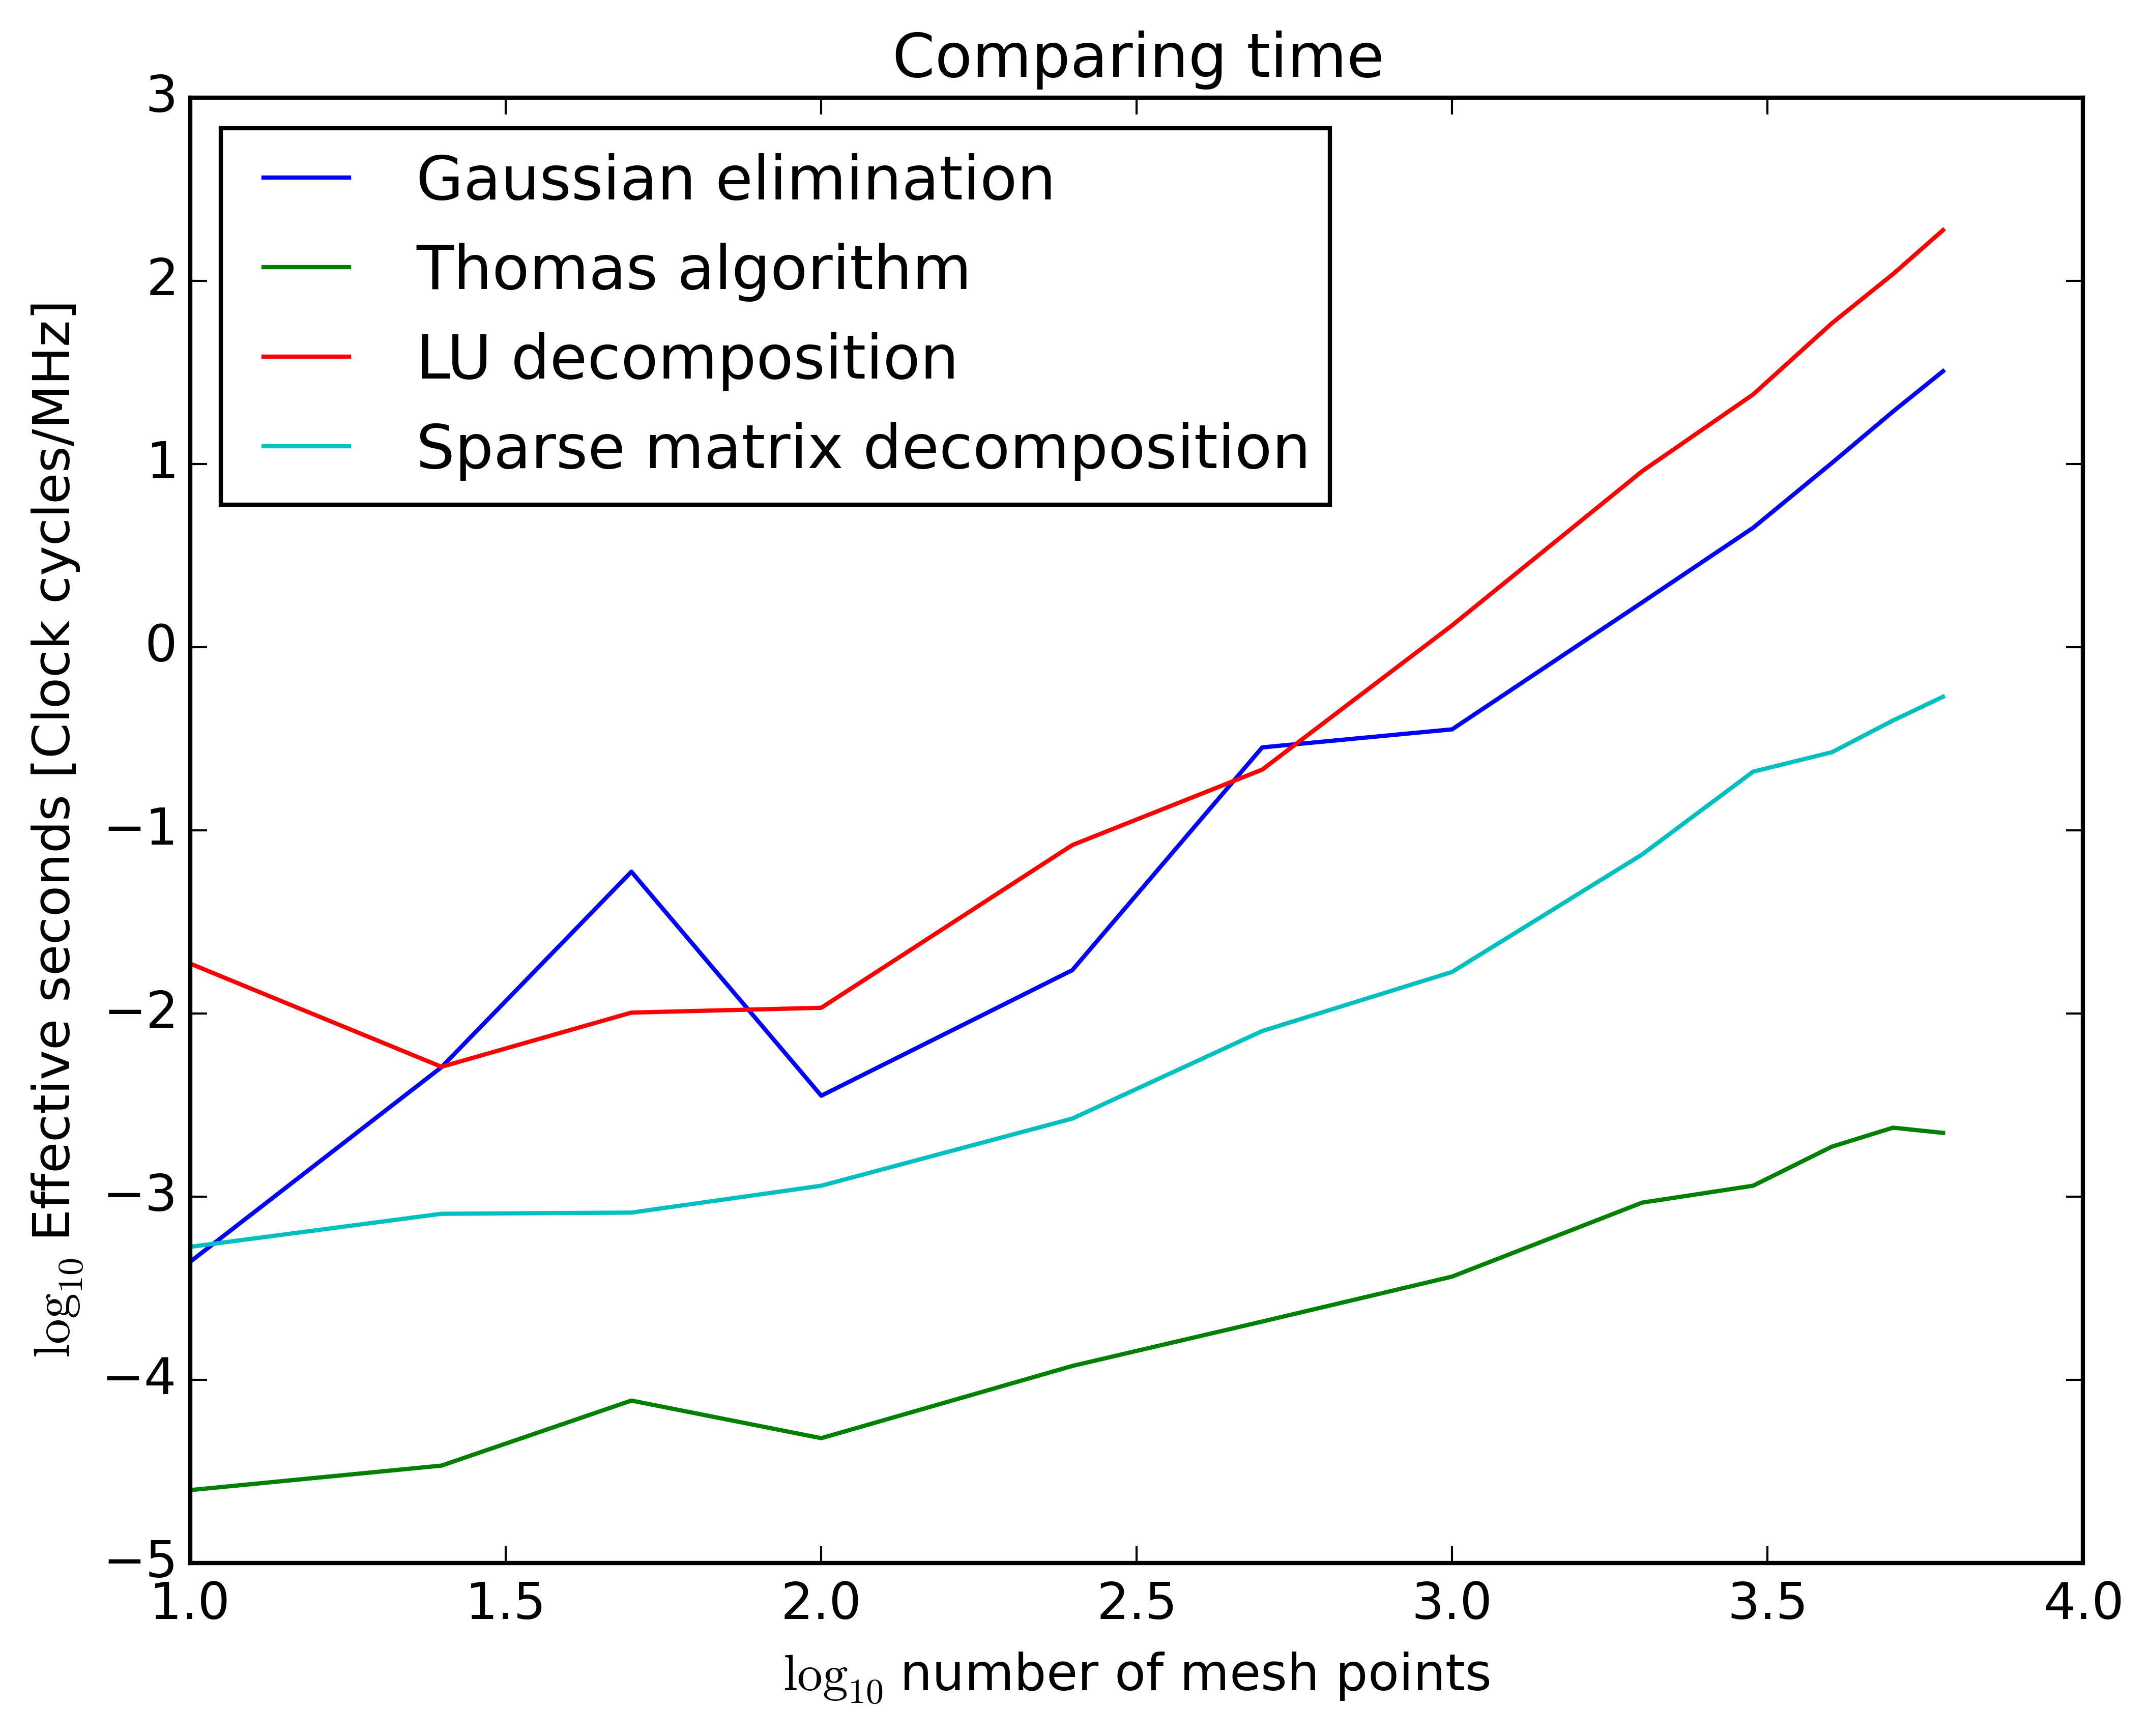
\includegraphics[scale=0.5]{Results/n_time.png}
  \caption{Time taken for the different algorithms plotted against 
  the number of mesh points}
  \label{fig:time}
\end{figure}


\subsection{Accuracy}

A table and figure of the error is included in table \ref{tab:err} 
and plotted in figur \ref{fig:err}. 

\begin{figure}[H]
\centering
  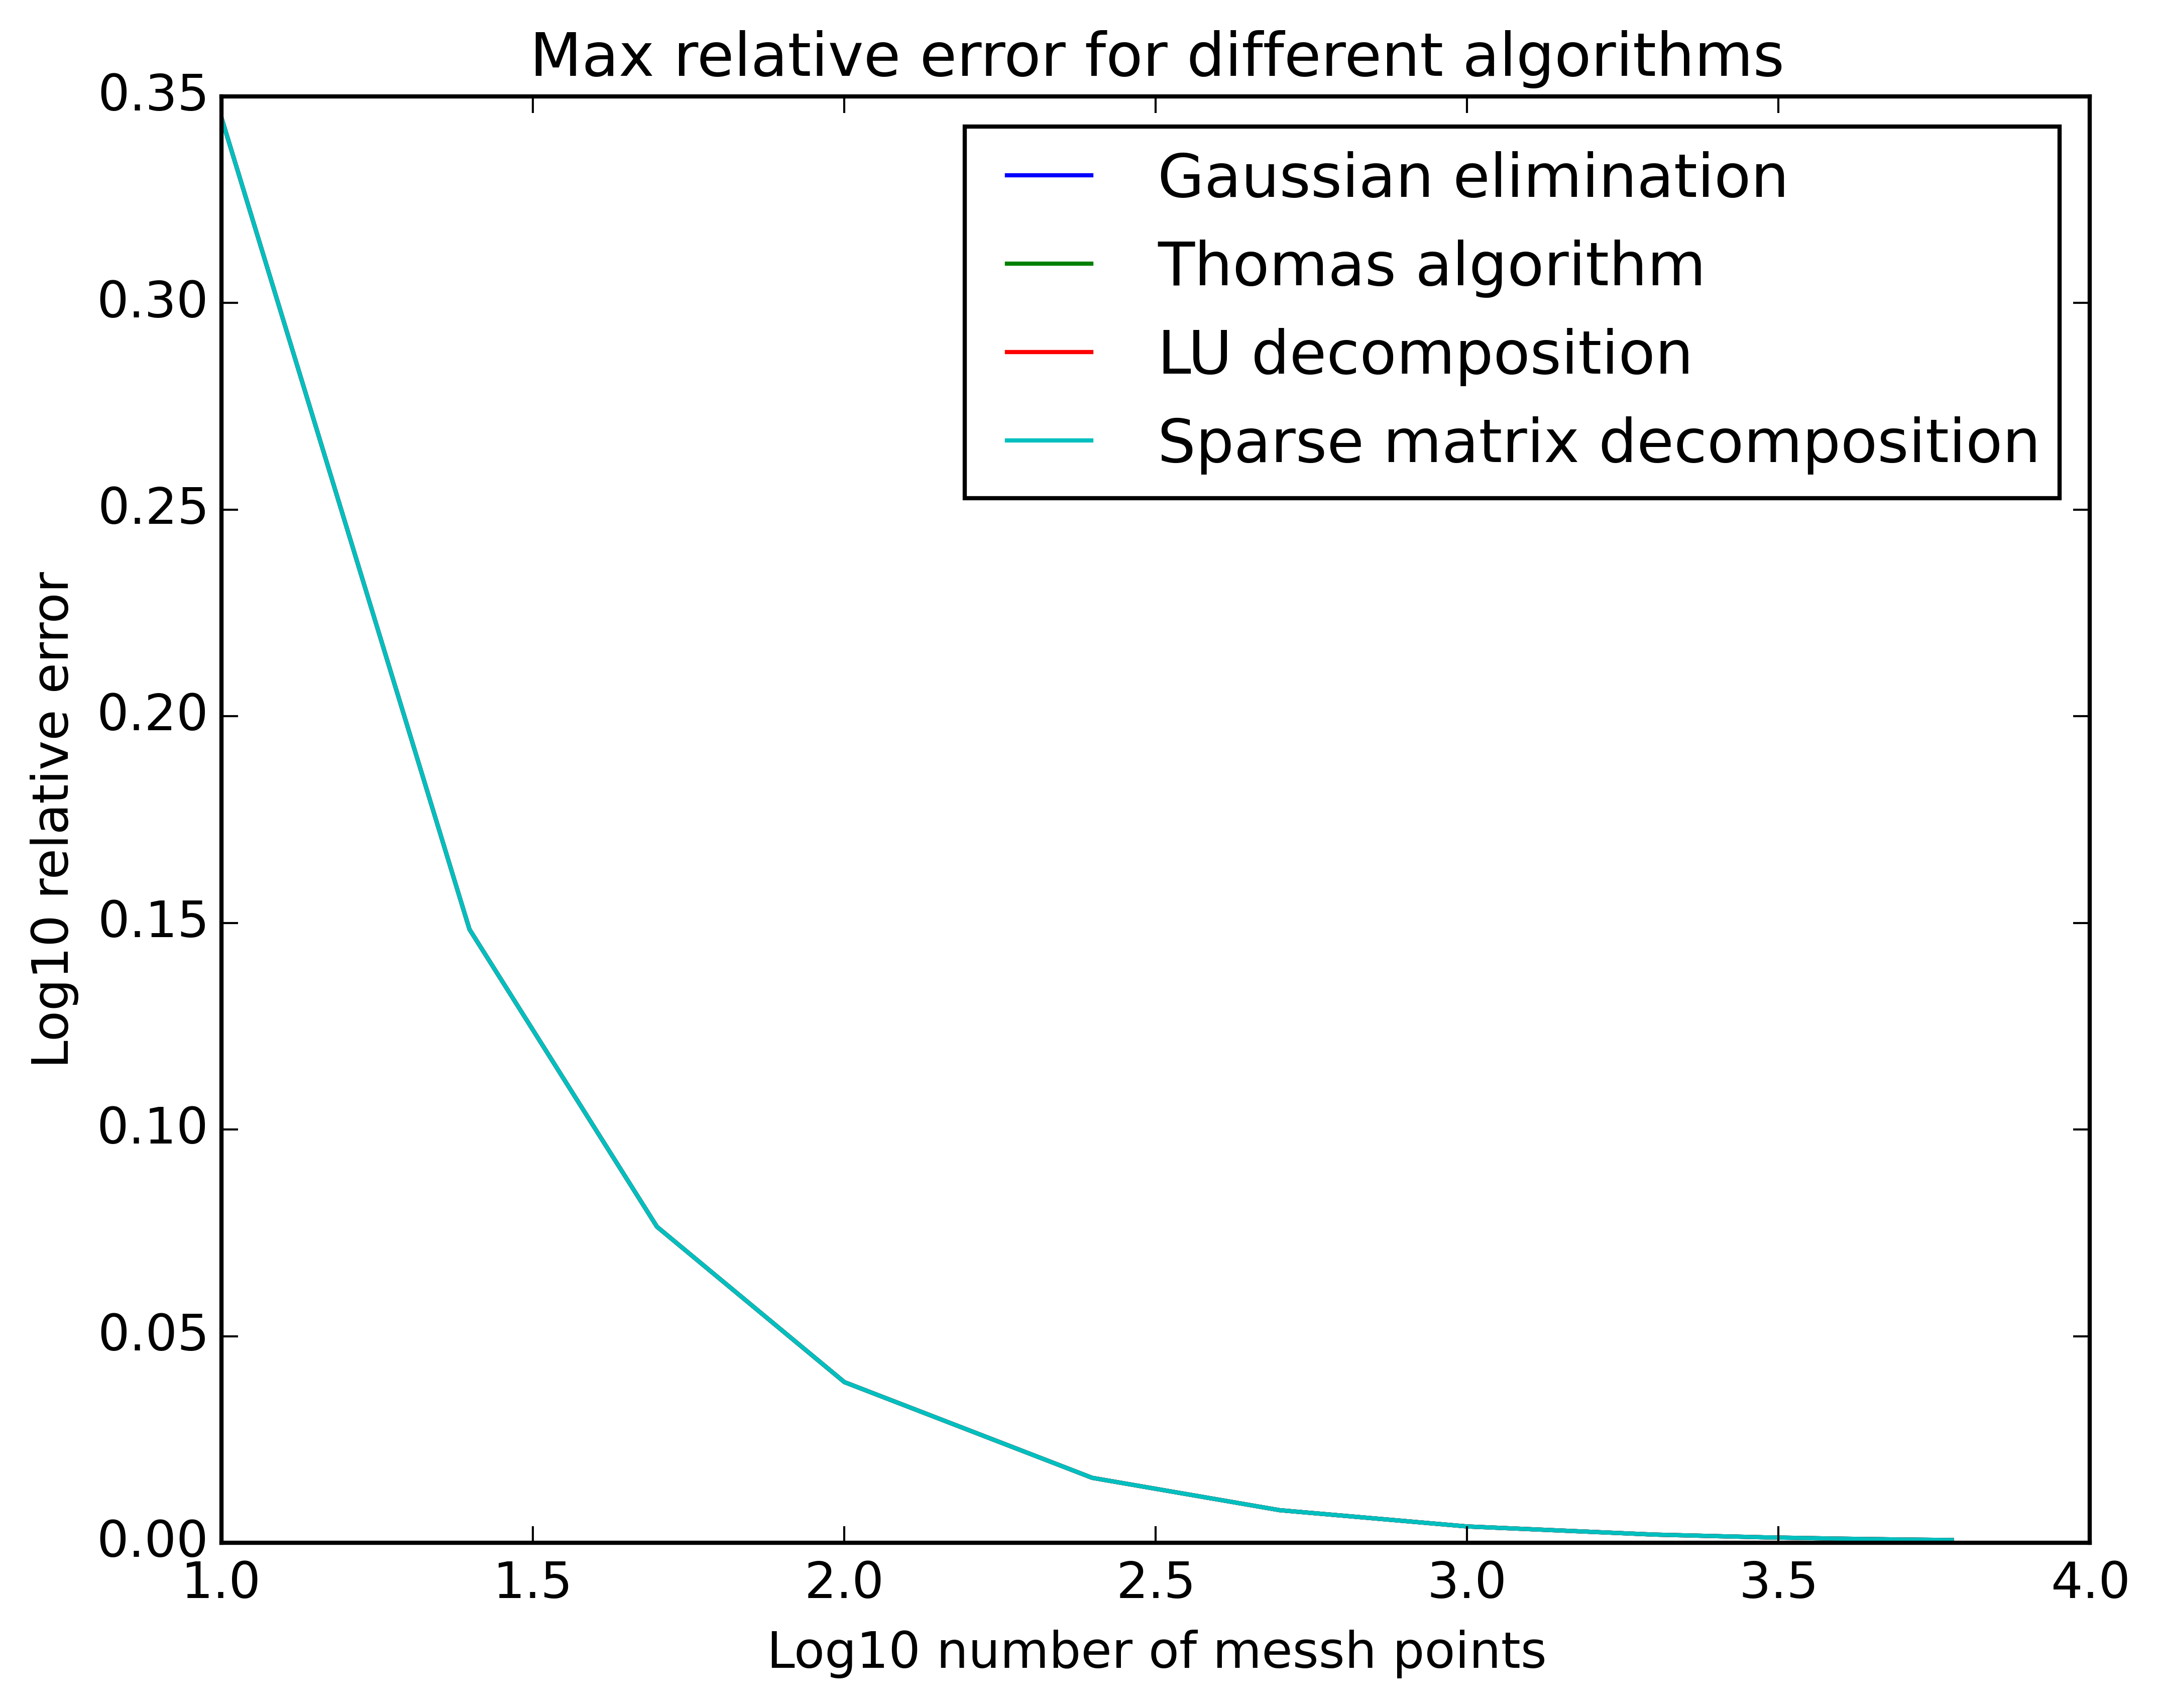
\includegraphics[scale=0.45]{Results/n_err.png}
  \caption{Relative error for the different algorithms plotted 
  againt the number of meshpoints }
  \label{fig:err}
\end{figure}

\begin{equation}
err = \max \left(\log_{10} \left(\mathrm{max}\left[
\frac{v_i - u_i}{u_i} \right]\right)\right)
\label{eq:error}
\end{equation}


The error is computed using \eqref{eq:error}.


The error is very similar, and is simply overplotted. This is saying that the methods
give the same results, and are using the same procedures. To obtain different(preferably better) convergence rates for the error, using a higher order approximation for the derivative is a way to go. That was not the goal for this project, but is worth mentioning. 

\begin{table}[H]
\centering
\caption{Comparing accuray of different algorithms for a different number
of mesh points. The error here is defined as $log_{10}$ of the maximum 
relative error. }
\vspace{3mm}
\begin{tabular}{|l|l|l|l|l|l|l|l|}
\hline
\multicolumn{1}{|c|}{ } & \multicolumn{1}{|c|}{Gauss Elimination} & \multicolumn{1}{|c|}{TDMA.} & \multicolumn{1}{|c|}{Sparse decompostion} & \multicolumn{1}{|c|}{LU decomposition}  \\
\hline
N & Error & Error & Error & Error  \\
\hline
10 & 0.34469208 &  0.34469208 &  0.34469208 &  0.34469208\\
25 & 0.14844317 &  0.14844317 &  0.14844317 &  0.14844317\\
50 & 0.07648232 &  0.07648232 &  0.07648232 &  0.07648232\\
100 & 0.0388765  &  0.0388765  &  0.0388765  &  0.0388765 \\
250 & 0.01571379 &  0.01571379 &  0.01571379 &  0.01571379\\
500 & 0.00788507 &  0.00788507 &  0.00788507 &  0.00788507\\
1000 & 0.00394968 &  0.00394968 &  0.00394968 &  0.00394968\\
2000 & 0.00197664 &  0.00197664 &  0.00197664 &  0.00197664\\
3000 & 0.00131816 &  0.00131816 &  0.00131816 &  0.00131816\\
4000 & 0.00098877 &  0.00098877 &  0.00098877 &  0.00098877\\
5000 & 0.00079109 &  0.00079109 &  0.00079109 &  0.00079109\\
6000 & 0.00065928 &  0.00065928 &  0.00065928 &  0.00065928\\
\hline
\end{tabular}
\label{tab:err}
\end{table}

\section{Concluding remarks}

Libraries for computational algorithms can be a great asset for scientists. However, one must not blindly belive that it is always the best option. To take into consideration how the algorithems work, and whether or not they are well suited for your specific problem is very important. The numerical experiments done in the project is good proof of that. Preforming a full Gaussian Elimination on a tridiagonal matrix is overkill. Just like you would not try to take out the rat in your basement using a nuclear bomb. 





\end{document}
